% Slug: four-of-diamonds
% Description: ?
% Author: Cisco
% Story: Cisco
% Test Data: Cisco
% Testers: ?
% Editorial: ?
% TempSlug: four-of-diamonds

% Please don't modify or delete TempSlug

\problem{Light Game}

Alice is replaying one of her favorite childhood platformers, \textit{Spongeboy: Skirmish for Scarborough Shoal}.  In this game, Spongeboy must defend his home from a ``robot'' invasion.  \textit{Supposedly}, it's said that the robots are an allegory for something, but Alice isn't quite sure what...  Metaphors are hard to decipher!

Aside from the main story, there are many puzzles which serve as side-objectives which can be completed for additional rewards.  One of these is the infamous \textit{Light Game}.

Spongeboy is dropped into a circular room, with $n$ lights arranged in sequence along the wall.  The lights are numbered $1$ to $n$ in the clockwise direction, and each light exists in one of two states: \textit{off} or \textit{on}. More formally, for each $1 \leq i \leq n$,
\begin{itemize}
\item for each $1 < i \leq n$, light $i-1$ is the left neighbor of light $i$ 
\newline (also, light $n$ is the left neighbor of light $1$);
\item for each $1 \leq i < n$, light $i+1$ is the right neighbor of light $i$ 
\newline (also, light $1$ is the right neighbor of light $n$).
\end{itemize}

Here is an example layout of the room with $n=8$.  Lights $3$ and $5$ and $7$ are initially on.
\begin{center}
    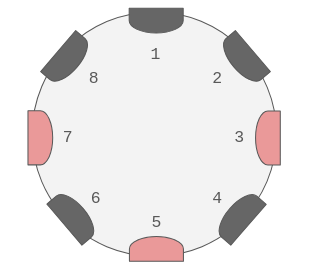
\includegraphics[width=0.3\linewidth]{img/light-game.png}
\end{center}


Each light is also a button that you can press.  When you press a light, the states of it and/or its neighbors may change, according to some seemingly random behavior.

Alice has a keen eye though, and deduced that the lights' behavior follows these consistent (if peculiar) rules:
\begin{itemize}
\item If you press a light where both its neighbors are off,
\newline both its neighbors are turned on
\item If you press a light where both its neighbors are on,
\newline its state is flipped \textit{and} both its neighbors are turned off.
\item If the pressed light has the same state as its left neighbor but not its right,
\newline the states of its two neighbors are \textit{both} flipped.
\item If the pressed light has the same state as its right neighbor but not its left,
\newline the state of the pressed light changes to be the same as its \textit{left} neighbor.
\end{itemize}
Here, ``flipping a state'' means: off lights become on, and on lights become off.

\newpage

Following the same example setup of $n=8$ lights from earlier (where initially, lights $3$ and $5$ and $7$ are on): if we press light $3$, then light $4$, then light $1$, then light $7$, we get the sequence of state changes illustrated in the diagram below.
\begin{center}
    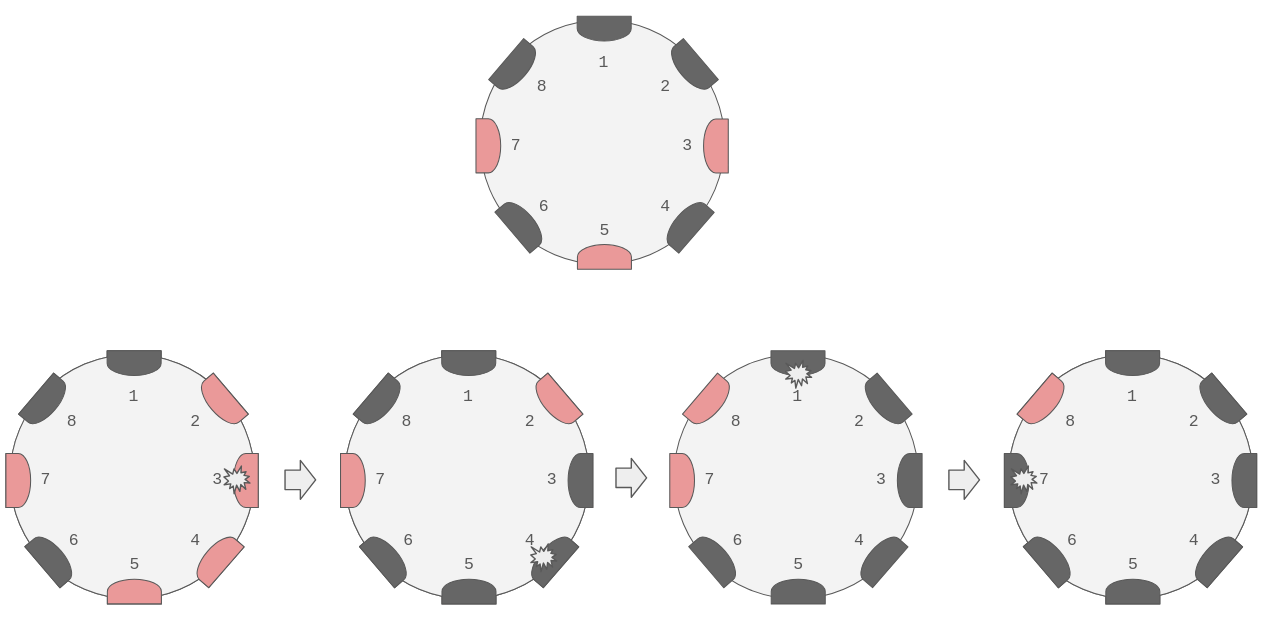
\includegraphics[width=0.85\linewidth]{img/light-press.png}

    \textit{We press light $3$, then press light $4$, then press light $1$, then press light $7$.}
\end{center}

You are given an initial configuration of lights, as well as the target configuration that Spongeboy must reach.  Does there exist \textit{any} sequence of button presses which achieves this goal?  If yes, please also construct such a solution.

\subsection*{Input Format}

Input consists of two lines, each containin a string of $n$ characters.  The first line represents the initial configuration, and the second line represents the target configuration.

The $i$th character is \texttt{1} if light $i$ is (or must be) on, and \texttt{0} if it is (or must be) off.  You are reminded that the room is \textit{circular}---despite the appearance of the input format, the first and last lights are actually next to each other.

\subsection*{Output Format}

Output a line containing \texttt{YES} if possible, and \texttt{NO} if not.

Then, if \texttt{YES}, output a solution.  First, output a line containing a non-negative integer $m$, the number of button presses in your construction.  Then, if $m > 0$, output another line containing $m$ space-separated integers, where each integer is from $1$ to $n$.  This encodes the instructions of which lights should be pressed, to be done in the order they are given.

Your solution must satisfy $m \leq 3 \cdot 10^5$.  Given the constraints, it can be shown that if a solution exists, then one satisfying $m \leq 3 \cdot 10^5$ exists.  If there are multiple possible answers, any will be accepted.

\newpage

\subsection*{Constraints}

\textit{Your program will only be tested on data that satisfies the following constraints.}

% Set to 10^5 in true bounds
\constraints{
    $3 \leq n \leq 100$ \\
    The input strings consist of \texttt{0} and \texttt{1} only.  \\
}

\textit{There is no need to validate in your program that these constraints hold.}

\subsection*{Sample I/O}

\begin{sampleIO}
\begin{verbatim}
00101010
00000001
\end{verbatim}
&
\begin{verbatim}
YES
4
3 4 1 7
\end{verbatim}
\end{sampleIO}

\begin{sampleIO}
\begin{verbatim}
000
111
\end{verbatim}
&
\begin{verbatim}
YES
3
3 3 3
\end{verbatim}
\end{sampleIO}


\begin{sampleIO}
\begin{verbatim}
01010
01010
\end{verbatim}
&
\begin{verbatim}
YES
0
\end{verbatim}
\end{sampleIO}


% \subsection*{Explanation}
